\documentclass[8 pt]{article}

\usepackage[utf8x]{inputenc}
\usepackage{dsfont}
\usepackage{amsthm}
\usepackage{amsfonts}
\usepackage{amssymb}
\usepackage{tensor}
\usepackage{mathtools}
\usepackage[T1]{fontenc}
%\usepackage[spanish]{babel}
\usepackage[cm]{fullpage}
\usepackage{graphicx}
%\usepackage{float}
\usepackage{bm}
\usepackage{setspace}
\usepackage{enumitem}
\usepackage{mdwlist}
\usepackage{parskip}
\usepackage{listings}
\usepackage{color}
%\usepackage{epstopdf}
\usepackage{tikz,datatool}
\usepackage{hyperref}
\usepackage{mathabx}
\usepackage{multicol}
\usepackage{eurosym}
\usepackage{caption}

\newcommand{\HRule}{\rule{\linewidth}{0.5mm}}

\AtBeginDocument{
  \let\myThePage\thepage
  \renewcommand{\thepage}{\oldstylenums{\myThePage}}
}

\newcommand{\gra}{$^\text{o}$}
\newcommand{\dif}{\text{d}}
\newcommand{\avg}[1]{\left\langle #1 \right\rangle}
\newcommand{\ket}[1]{\left| #1 \right\rangle}
\newcommand{\bra}[1]{\left\langle #1 \right|}
\newcommand{\bket}[2]{\left\langle #1 \middle| #2 \right\rangle}
\newcommand{\der}[2]{\frac{\text{d} #1}{\text{d} #2}}
\newcommand{\prt}[2]{\frac{\partial #1}{\partial #2}}
\newcommand{\dert}[3]{\frac{\text{d}^#3 #1}{\text{d} #2^#3}}
\newcommand{\prtt}[3]{\frac{\partial^#3 #1}{\partial #2^#3}}
\newcommand{\dl}{\mathcal{L}}
\newcommand{\dha}{\mathcal{H}}
\newcommand{\vol}{\text{vol}}
\renewcommand{\vec}[1]{\pmb{#1}}

\DeclarePairedDelimiter\ceil{\lceil}{\rceil}
\DeclarePairedDelimiter\floor{\lfloor}{\rfloor}

\newenvironment{Figure}
  {\par\medskip\noindent\minipage{\linewidth}}
  {\endminipage\par\medskip}

\begin{document}

\begin{minipage}{\textwidth}
    \centering
    \Large \textbf{\textsc{Homework 4: Correlated Statistical Arbitrage}}
    \vspace{0.5cm}

    \small \textsc{Francisco García Flórez, Joris van Lammeren, Wouter Varenkamp}
    \vspace{0.5cm}

    \begin{minipage}{0.8\textwidth}
      \textbf{Abstract.} In this homework statistical arbitrage is used to extract profits from changes in the market pricing of two stocks. As is common with actual industry sectors several similar stocks behave similarly over time, formally known as correlated stocks. In this case we consider two banks, EUR\_CBK and EUR\_DBK, and by using statistical arbitrage with extra information from the correlations we will make a certain profit.
    \end{minipage}
\end{minipage}

\vspace{0.5cm}

\begin{multicols*}{2}

  \section{Trading robot}

  This trading robot is more complex than the previous one used to benefit from pure arbitrage, since we need to study and understand market fluctuations and guess how is the price going to change at a later point in time. First we will introduce the fundamental concepts on which the robot is based and then briefly explain how it all works together. Finally, results and further improvements will be discussed.

  \subsection{Trades}

  In this robot, a \textbf{trade} is a set of transactions associated with one ISIN consisting of triplets containing the price, volume and time: $(P_i, V_i, t_i)$. Note that the volume can be negative, meaning we sold that volume. Using this basic unit, our robot will have two modes of operation, namely \textbf{adding new trades} and \textbf{completing active trades}.

  Moreover, each trade will only consist of one transaction initializing the trade, and every subsequent one will reduce the position given by the first. Therefore, the side of a trade is simply defined by the volume of the first transaction: $\text{sign}(V_0)$.

  \begin{itemize}
    \item \textbf{New active trade.} We can differentiate between two kind of trades, those which are still active and those that has been completed. Each one is defined by checking if the added volume is zero: $\sum_i V_i = 0$. If it is, then it is considered \emph{completed}, and \emph{active} otherwise.

    Adding a new active trade means finding a right moment in time to buy or sell stock and initialize the trade with that transaction, in the hope that the price will get higher or lower allowing for some profit.

    \item \textbf{Completing active trades.} Once we have created a new trade, we need to check whether or not is profitable to reduce our position in the market, by computing the expected profits of the trade at a certain moment in time. This is done by computing the following value

    \begin{equation*}
      P_{\text{exp}} = P_{\text{prop}} \sum_i V_i - \sum_i V_i P_i ~~,
    \end{equation*}

    where $P_{\text{exp}}$ is the expected profit and $P_{\text{prop}}$ is the selling or buying price proposed by the market. If this results in a positive amount, we can consider proceeding with the transaction, and also allows us to sort each active trade in terms of expected profits, fulfilling the most profitable ones before the others.
  \end{itemize}

  Having defined the main modes of operation, we remark that the number of active trades is not limited, however there are several considerations we need to issue for the program to make any profits. First of all, this model (just by itself) relies on having enough time to fulfill almost every active trade to make profits, since even though our position in the market at some time can be zero, our profits may in the negatives because we are investing in buying stock for later transactions. Later we will discuss several possible ways to reduce this effect.

  As a final remark, we can now refer to \emph{completed trades profits} as the profits made only from completed trades, as a measure of how well the program is working excluding other factors like unwinding.

  \subsection{Detecting price peaks}

  In the last section we describe the idea of trading at the right moment in time, and for that we need to detect which ones those are. In the first approach, without using any correlations, we can look at the actual market and compute a value for the stock, which will move following what we can consider a Brownian motion. However, this is a mathematical object difficult to work with, so to be able to detect peaks using standard tools like derivatives we need to remove part of this randomness and extract a continuous value.

  For this we will use a modified version of the \emph{Holt-Winters algorithm}, also known as triple exponential smoothing. Fundamentally, it works as a high frequency filter on the fluctuations of the market value, resulting in a smooth trajectory that can be differentiated. We use a modified version without seasoning or forecasting, but it also computes the smoothed second derivative of the price, so that we can know if the peak is a maximum or a minimum.

  Another benefit of this approach relies on providing us with three parameters, $\alpha, \beta, \gamma \in [0, 1]$, which we can adapt to better approximate the actual price. Values closer to zero correspond to using more past values to compute the current average, while a value of one just returns the real market value. These three values can be further optimized by several approaches, mainly \textbf{initial values optimization} and \textbf{runtime adaptation}.

  In \textbf{initial values optimization} we run the algorithm over the feed data several times with different values for these parameters, choosing the ones that maximize the profit. On the other hand, \textbf{runtime adaptation} modifies them during the simulation. Each approach can give different results depending on the actual behavior of the market, however in our case we can expect the former to be good enough, since the length of the feeds is not significant.
  Finally, we can apply this smoothing to any quantity related to the market, but we will mainly use it to determine the ask and bid prices, the total volume of the book and to store the real ask and bid values of the stock. In the program however it has been generalized and can be used for any function using values from the book.

  \subsection{Stop-Loss algorithm}

  As we mentioned before, this simple algorithm will fail to make profit because some active trades get ''stuck`` when we get some position at a value that won't make any profit at a later time. This situation can easily happen when there is a significant dip in the price and we got a negative position at the peak, rendering it unable to make any profits.

  There are several strategies we can follow to reduce the effect of this situation on our profits, but we can categorize them in two groups: \textbf{volume limiting} and \textbf{stop loss}, however both can work in parallel. The former relies in trying to estimate the right amount of stock we should trade in the beginning so that the volume is not high enough for the market to absorb if we want to get rid of our position. The latter, on the other hand, estimates how much losses each active trade is having and tries to fulfill it before they are too large.

  In our robot, both are implemented in a simple way. The position gained is limited by the volume contained in the first entries of the book, while the stop loss checks for active trades with a relative loss larger than a set value and tries to complete them.

  Another relevant source of losses comes from the end of the feed, since our position at the end has to be zero. If we have a significant position when the feed ends we risk two problems. First, we don't know if the market has that volume available so we can remove our position, so we can get stuck with some stock. Second, even if the market can take it, we can incur in significant losses because of a dip in price. To reduce this, we have to be aware of how long the feed is and try to reduce our position gradually, meaning that near the end of the feed we will be making less profits but we can get rid of our temporal position without significantly affecting the rest.

  \section{Results}

  In Figures \ref{fig:results_1}, \ref{fig:results_1_closer} and \ref{fig:results_1_closer_b} we can see the actions of the robot, where the red continuous line is the ask price level (computed by the smoothing algorithm), discontinuous red line is the market ask price (first entry of the book), and similarly for blue lines, being the bid price in this case. Dots, red and blue, represent buying and selling respectively, so we can know when exactly the program is detecting a peak.

  Since in this case we have limited the amount of stock we buy, we can see several intervals in which nothing seems to happen, and is in this periods when the stop-loss algorithm should kick in and fulfill previous trades to keep new ones coming. We haven't included correlations in the algorithm yet, but the most significant contribution from them would be that instead of buying or selling not exactly at the peak, we can actually predict where the peak is going to be, and then stop loosing a small amount on each trade.

  We can also clearly see in this plots one of the problems we have to work with: the bid volume is on average almost an order of magnitude smaller than the ask volume. This means that we need to be very careful buying stock, since it is quite easy to get stuck with it.

  Now, since there are still a few problems with the algorithm, by looking at the completed trades profits:

  \begin{verbatim}
  Completed trades profits:

    DBK_EUR:     486.96
    CBK_EUR:      67.55
    Total:       554.51
  \end{verbatim}

  We can see that completed trades are actually making profits, however the final profits are \texttt{-126.92} (assuming we unwind successfully), mostly because we have bought stock to compensate the total position by opening active trades that didn't get fulfilled.

  \section{Conclusion}

\end{multicols*}

\section{Appendix}

\begin{Figure}
  \begin{center}
    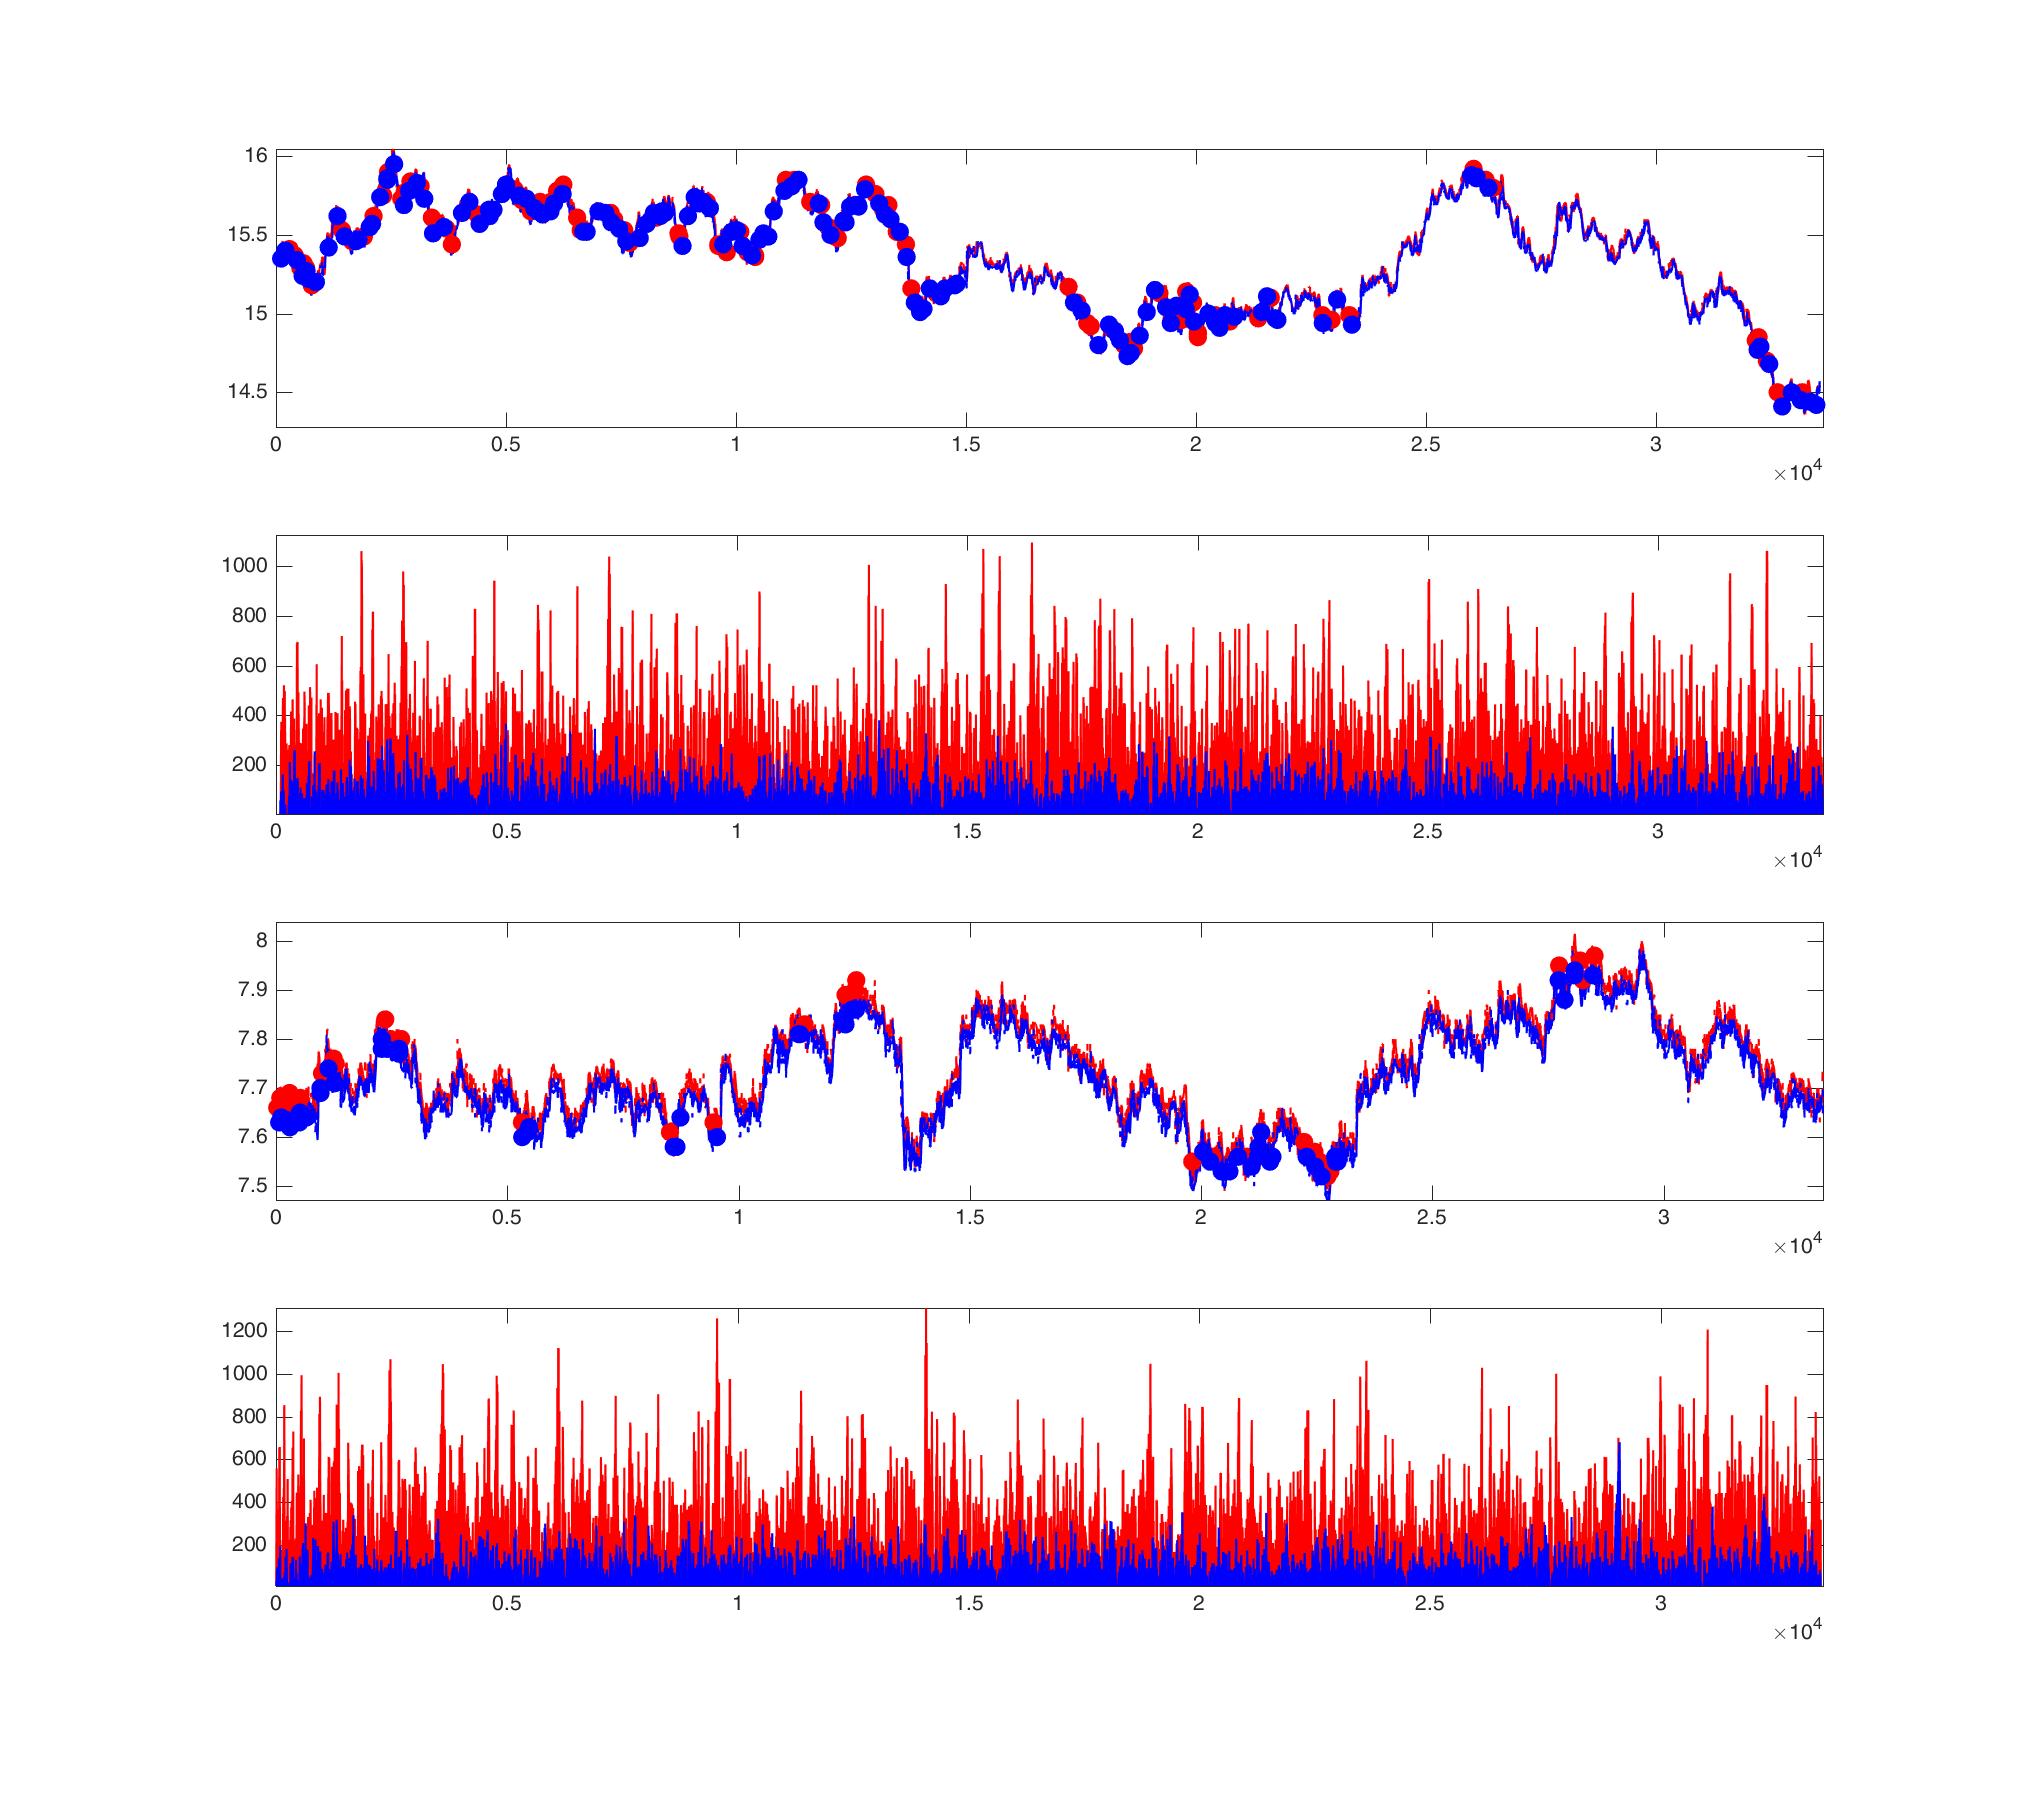
\includegraphics[width=\textwidth]{graphs/result_CBKDBK1.eps}
    \captionof{figure}{Results after running the program for the first feed. The first and second plots correspond to the ISIN DBK\_EUR, ploting price value and volume respectively, and the last two correspond to CBK\_EUR.}
    \label{fig:results_1}
  \end{center}
\end{Figure}

\begin{Figure}
  \begin{center}
    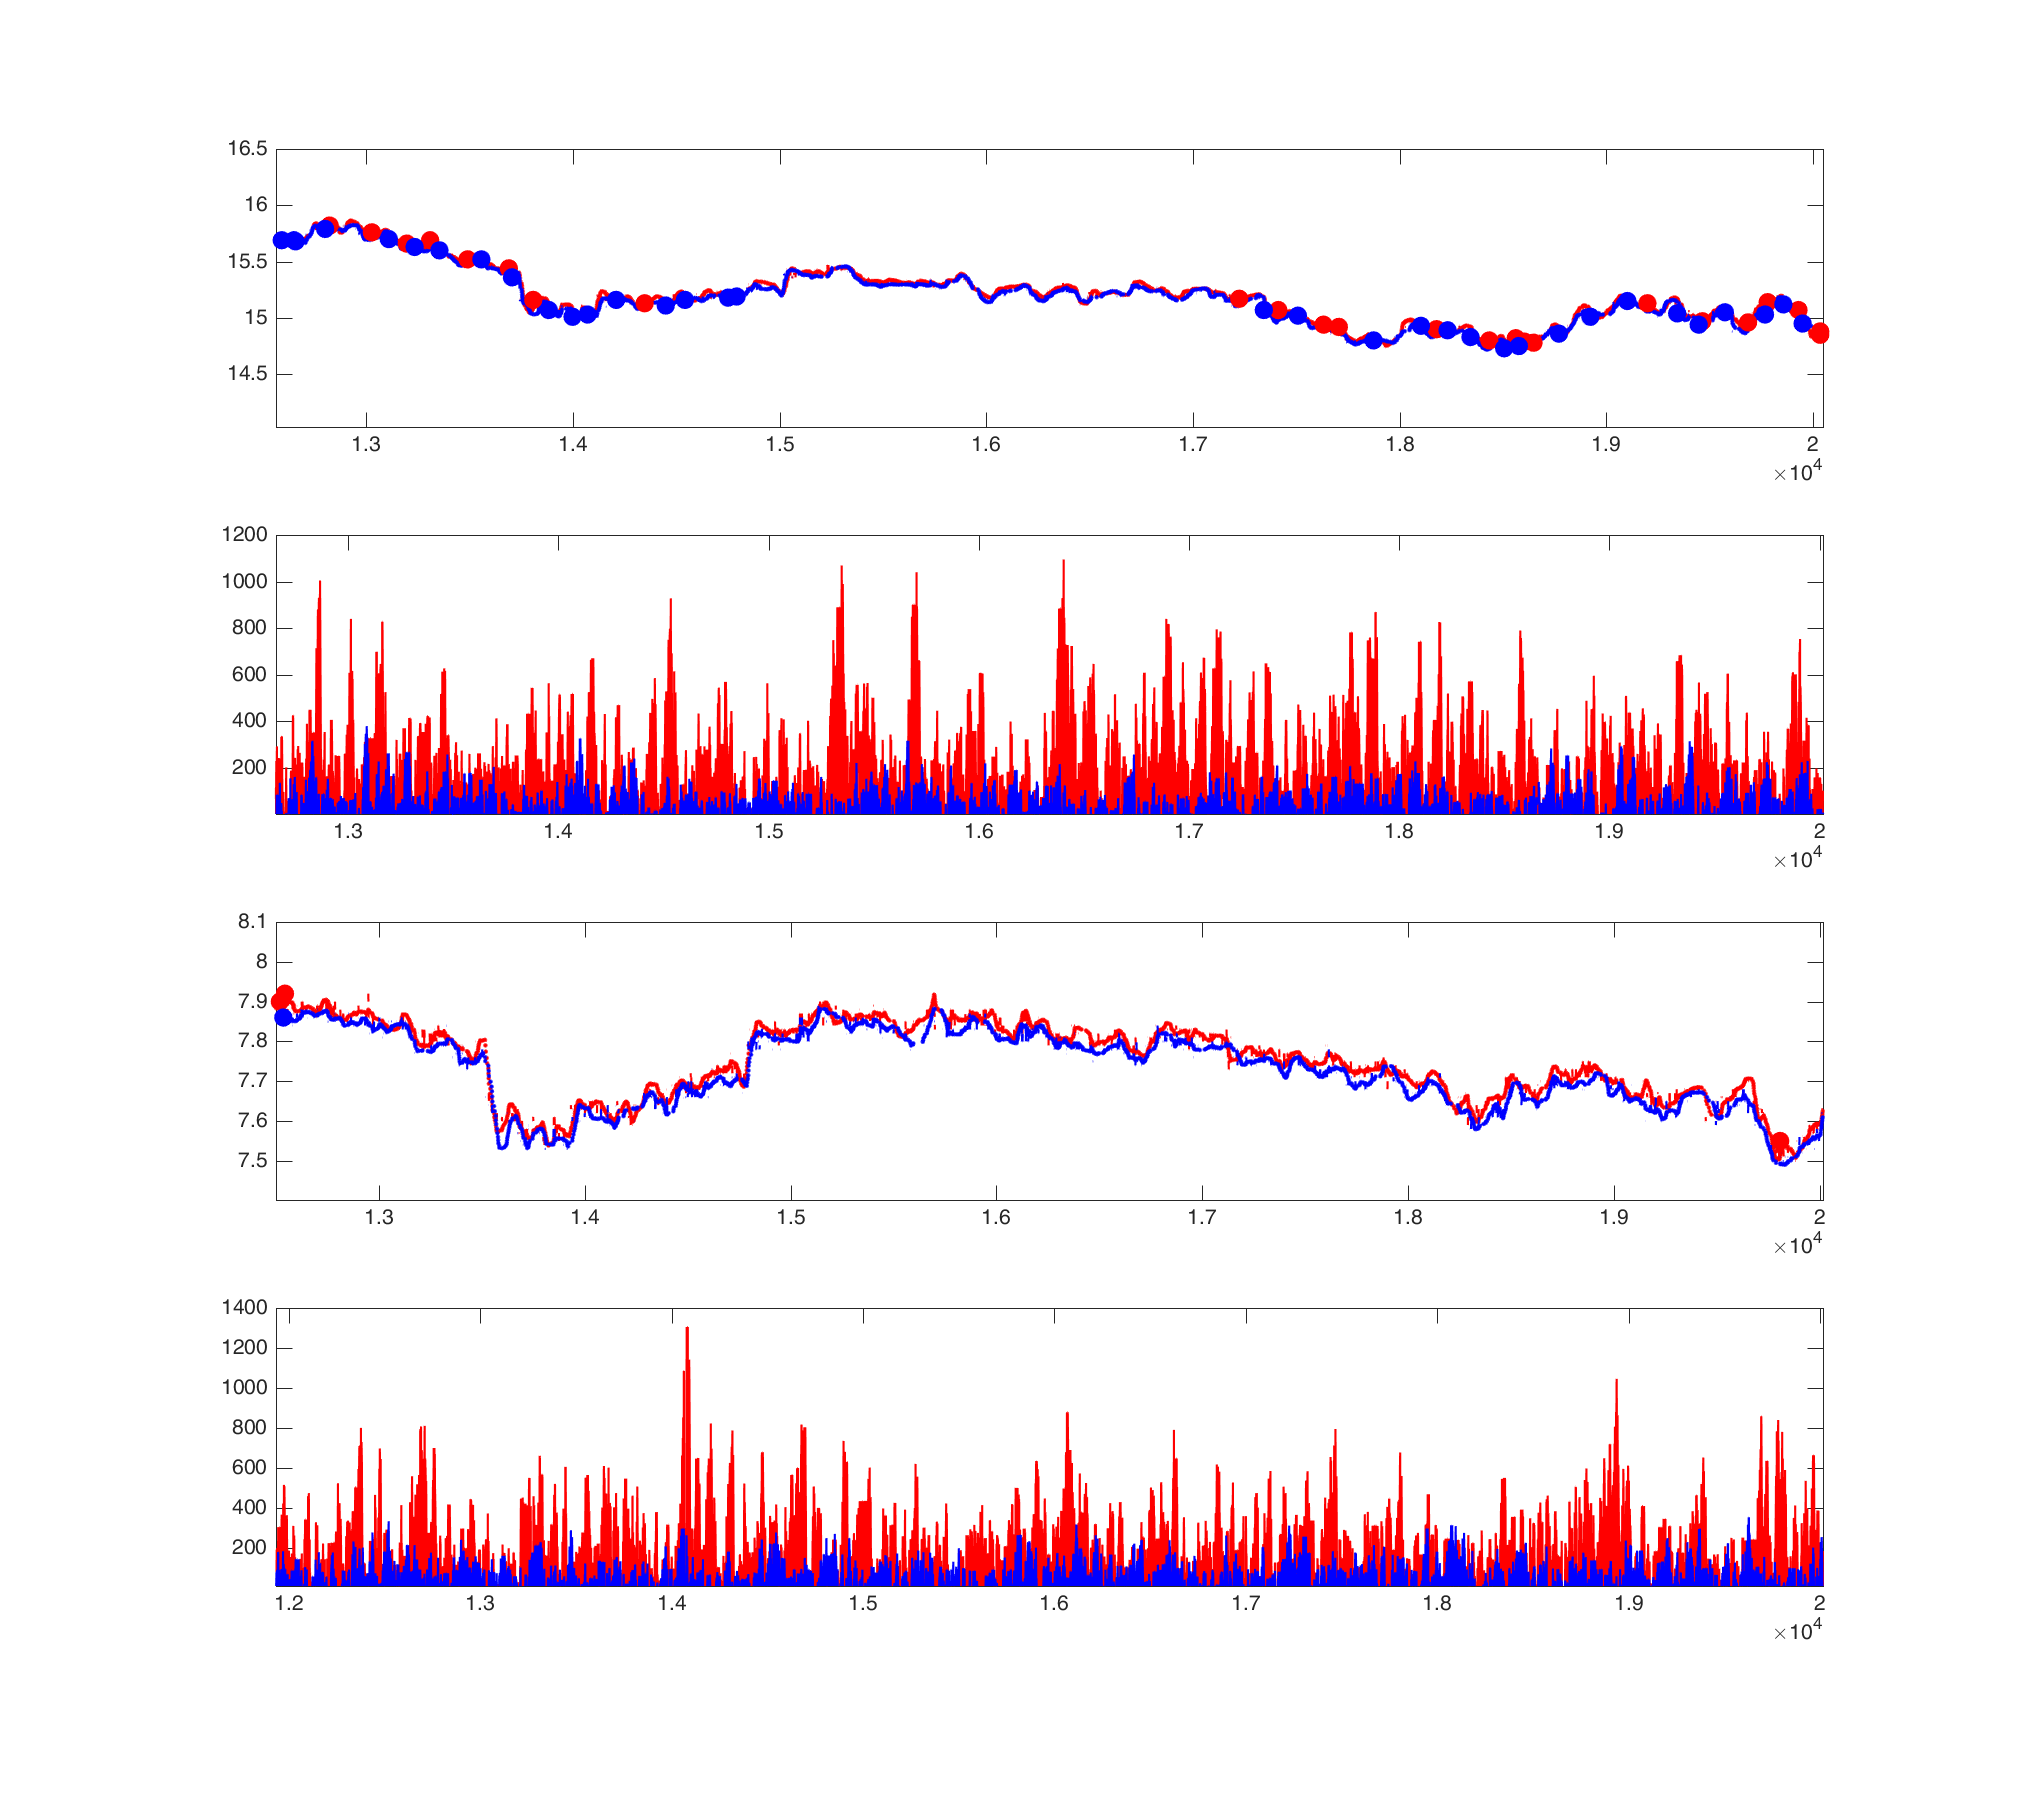
\includegraphics[width=\textwidth]{graphs/result_closer_CBKDBK1.eps}
    \captionof{figure}{Results after running the program for the first feed, closer look.}
    \label{fig:results_1_closer}
  \end{center}
\end{Figure}

\begin{Figure}
  \begin{center}
    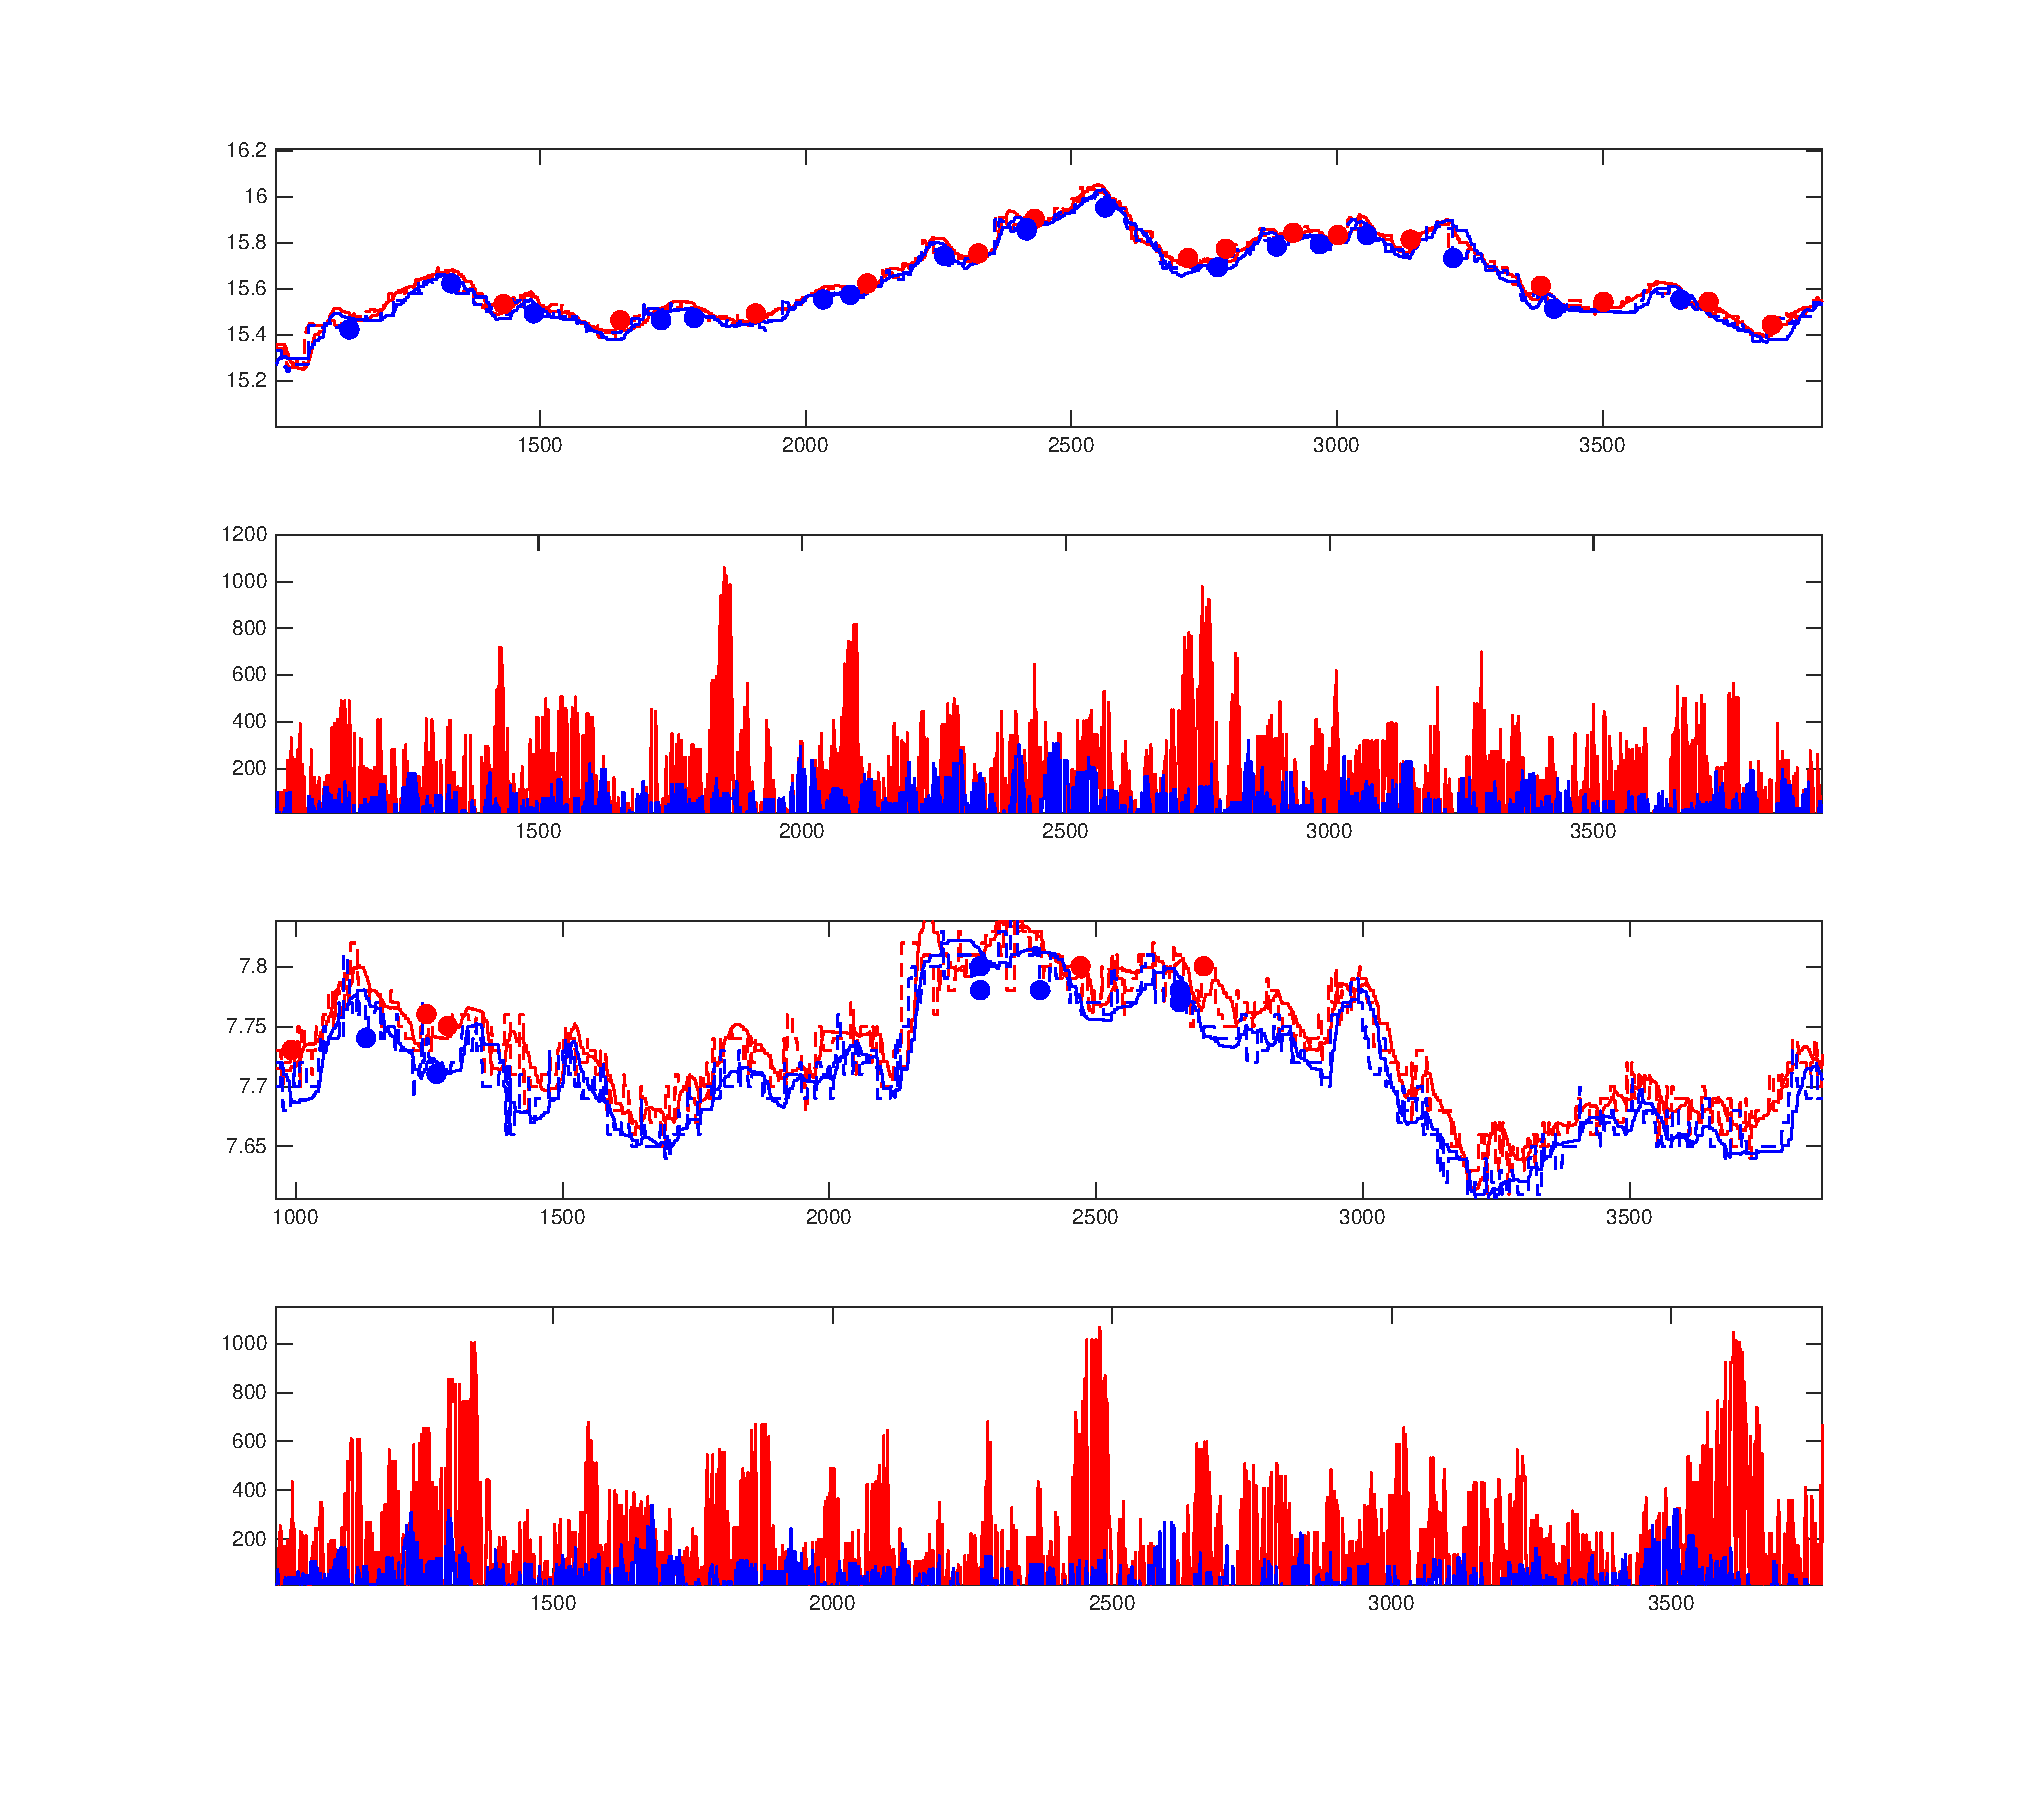
\includegraphics[width=\textwidth]{graphs/result_closer_b_CBKDBK1.eps}
    \captionof{figure}{Results after running the program for the first feed, another closer.}
    \label{fig:results_1_closer_b}
  \end{center}
\end{Figure}

\begin{thebibliography}{28}
\raggedright
\addcontentsline{toc}{section}{Bibliography}

\bibitem{Wilmott} P. Wilmott et al, \emph{The Mathematics of Financial Derivatives}, 1995.

\end{thebibliography}

\end{document}
